\documentclass[12pt,a4paper]{book}
\usepackage{graphicx}
\graphicspath{ {./images/} }

\author{Simone Pernice}
\title{Penthode 1.20 User Manual}
\date{1st September 2018}

\begin{document}
\maketitle
\chapter{Introduction}
Pentode design begun on 3rd December 2016 by Simone Pernice. When Pentode was born there was not any tool to design a power distribution.  
Pentode names comes from PowErTreeDEsigner. Pentode was a device used as transistor in high quality audio pre-amplifier of the old age before the solid state transistor coming.\\
Pentode is open source however its development takes a lot of time. If you make a donation you can grant its manual, get help, request features, etc.\\
Pentode is a tool to design, simulate, draw the high level power distribution of a device. The power distribution, sometime called power tree of a device, shows how the power is delivered from the sources (battery, DC supplier), converted to the required voltages, provided to the loads (display, CPU, ...).\\
Pentode session usually begins loading the high level net list of the device. The user can prepare that net list describing the device power architecture. That is just a starting point, it is also possible begin from an empty net list and interactively: add, modify and delete components of the power distribution. It is possible to simulate the power distribution looking for components running out of specification, plotting their current and voltage waveforms. It is also possible compute the power tree BOM (bill of material) cost. If the result is not satisfying the power tree can be modified and simulated again. When the iterations are completed it is possible to save all the history commands given to continue from there later.\\
After starting Pentode, the user runs can interactively: 
\begin{itemize}
\item Commands to simulate the voltage and current up to the steady state: the simulation reporting components working out of specification
\item Simulate same circuit several times stepping some parameter to find the best performance
\item Draw a nice power tree diagram showing the currents/powers balance on pdf/svg file
\item Plot node transient voltage and gate current waveforms on png/jpeg file
\item Change component parameters interactively to improve the design, delete or add components 
\item Iterate through loops and lists, check conditionals, manipulate variables and perform basic calculus to automate repetitive tasks
\item In the net-list commands or interactively, it is possible to modify the power tree to test new configurations: modified components properties and adding or deleting components
\end{itemize}
Pentode workflow is showed in the next picture:\\
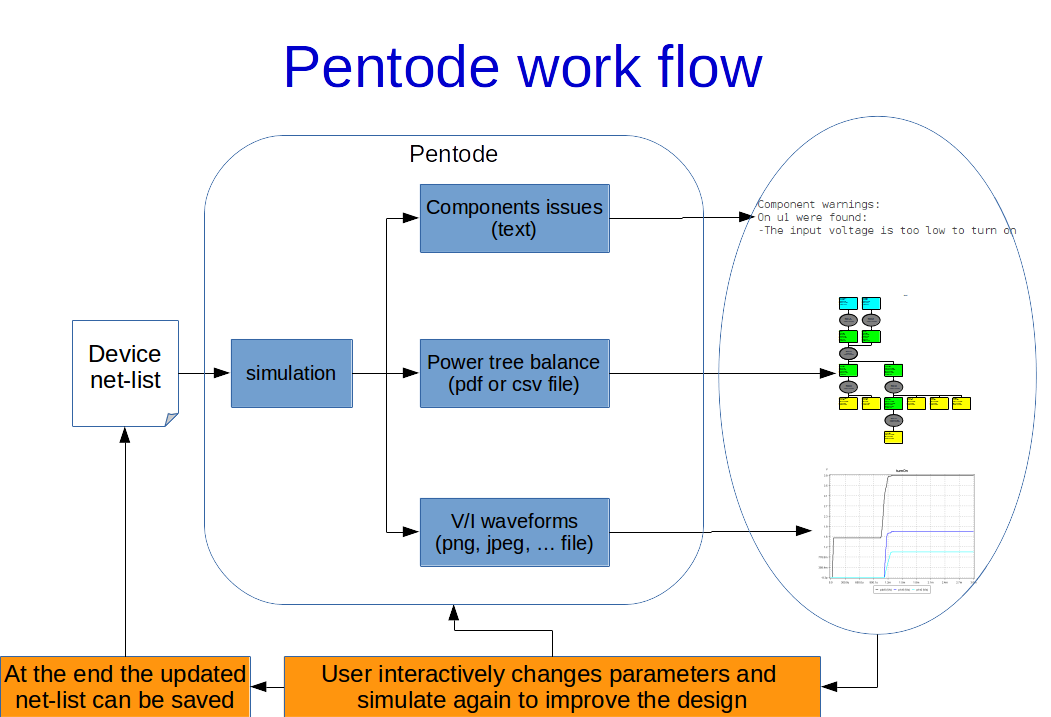
\includegraphics[width=\textwidth]{PentodeWorkFlow.png}\\
The main concerns designing the power distribution of a new device are:\\
\begin{itemize}
\item Efficiency: it is good to minimize the input power especially on portable devices to provide long battery life. High efficiency can be achieved with:
\begin{itemize}
\item Scalability: the capacity to turn off the not used regulators in order to reduce the energy waste
\item Standby current: is the special case of scalability where almost all components are turned off and the device drains a negligible current to preserve the battery charge.
\end{itemize}
\item Cost: the device has to be the cheapest possible but that goes against efficiency because usually more efficient converters are more expensive. To achieve the optimum it is required to compare several solutions.
\item Ratings: every source, converter and drain has to work within its specification
\item Correct suppliers turn on and off sequence: that is very important when the components linked together use several rails 
\end{itemize}
Usually the power distribution design requires to:
\begin{itemize}
\item Define all the user cases: Standby, WiFi, Video + WiFi, Video + Ethernet, ...
\item Define the most suitable power trees. That is a trial and error procedure which requires to draw on paper the most promising architectures 
\item Compute the cost of every architecture 
\item For each couple: use case – architecture the designer has to evaluate the efficiency computing the power balance  
\item Choose the best trade off between cost and efficiency 
\end{itemize}
Pentode can automate and simplify all those steps to get a faster and more accurate result.\\
\chapter{Basics}
This chapter describes Pentode basics. Pentode simulate a \emph{device}. A device is  made by a net of \emph{electric components} linked to the \emph{nodes} of that device. There are two main types of electric components \emph{node} and \emph{black box}. \\ 
Pentode session begins reading an input file (.ptd extension). Usually that file describes the device components and their links, however it is possible to begin with an empty file and adding interactively all the components required by the architecture. Each line is a command to be executed: if the command is the description of a component it is added to the device.  A component is defined by its unique label, type (supplier, converter, drainer, etc.), by its parameters (output voltage, etc.) and interconnections to the nodes of the devices. After the device is defined a set of commands to simulate and show its results are used. Once the commands in the input file are executed, it is possible to continue interactively to write commands or modify the device at Pentode's prompt. When the target result is achieved a \emph{save} command will add to the input file the new lines added interactively after its loading. Pentode session ends with the \emph{quit} command.\\
\section{Basic Components}
Pentode simulates a \emph{device} made by a net of \emph{electric components} linked to the \emph{nodes} of that device. There are two main types of electric components \emph{node} and \emph{black box}. Every time an input line describing a component is found, it is added to the device. Pentode always try to add a new component although something is not understood due to syntax errors which are reported.\\
\subsection{Node}
The nodes are defined by their label and capacitance value. It is optionally possible to set their simulation begin voltage to use to start the simulation. By default the simulation begins with all nodes at 0V.  Nodes are usually defined automatically when the black box is declared because it is required to write the nodes at which it is linked to. Nodes label are defined by user. Nodes save their voltage history to be plotted after the simulation if required. Its electrical capacitance stores or provides charge when there is a mismatch among the current magnitudes entering and exiting on the node.\\
\subsection{Black box}
The black boxes is defined by its label and the link between its \emph{gate}(s) and the nodes. Every black box has one or more \emph{gate}s through which the current flows to the device's nodes. The gates at the same voltage are linked to the same node. Gates store the black box current histories which can be showed after the simulation.\\
Power suppliers and drainers have just one gate (to output or input their power), while converter at least two (power flows from input to output). Pentode names gates by a sequential number: 0 for single gate, 0 is input and 1 output for dual gate. The currents flowing through those gates are defined by not-linear time-variant behavioral-equations depending on the voltage of the nodes at which they are linked to. By definition the current entering a component is positive and negative if it exits. \\
The behaviors of the most commons electric components are already stored in Pentode. The user has to customize their characteristic setting \emph{parameter}s like the output voltage of a voltage regulator. Almost all parameters have a default value to be used if it is not set by the user.\\
The black boxes providing power are called \emph{source}. They have just one gate (number  0) to output their power. For instance a source can be a DC adapter or a battery. Their behavioral model takes into account of parameters like: internal resistance, maximum current, voltage waveform (for time-variant source), etc. The purpose of those parameters is to simulate the real component behavior.\\
The \emph{converters} have at least an input (gate 0) and an output (gate 1) usually. There are also controlled converter with a third gate (2) working as enable. Their purpose is to convert the power from the input gate to the output changing its voltage for instance. Examples of converters are diodes, switches, LDOs, buck or boost converters. Their behavioral model takes into account of parameters like: load and line regulation, maximum current, minimum input voltage, quiescent and disable current; for switching converters: switching and resistant current loss, working mode (PWM or PFM), etc.\\
The \emph{drains} use the power provided by sources and converters like LED or resistor. They have just the input gate (0). Their behavioral model takes into account of parameters like: minimum operating voltage, equivalent resistance, current or power, etc.\\
\section{Commands}
Once the power architecture is defined some commands are used to play with it. \\
The work begins simulating the power architecture. The second step is to show the simulation results to be checked for problems. If some problem is found there it is possible to modify the power architecture to restart a new cycle. \\
\subsection{Simulate Commands}
Pentode performs a time domain simulation based on Runge Kutta 3 as default. It is possible to use several integration algorithms setting a parameter: increasing their complexity improves the result at expense of calculation length. The simulation begins from the initial state of the node voltages (0V by default).\\
With the \emph{simulateTransient} several node voltages and gate currents during the simulation are stored and the simulation ends at the user defined time. That simulation is useful to verify power on and off sequences and other dynamic behavior looking at their voltage and current plots.\\
It is also available a \emph{simulateSteady} command which is a transient simulation automatically interrupted when the node currents mismatch is below a given threshold or if the maximum user defined simulation time is reached. In this simulation only the last voltage and current state is saved. This simulation is useful to check for power balance, efficiency and power consumption in several cases. \\
At the end of simulations all the components are checked against strange behavior: like a reverse biased diode or regulator exceeding its maximum current. \\
\subsection{Show Commands}
Once a simulation is run it is possible to \emph{draw} a power tree. The power tree is a graphical picture of the last state computed on the (usually steady) simulation. The black boxes are drawn as squares with color and placement depending on their nature. Sources are drown on top in light blue boxes, converters are green in the middle and the drainer are in yellow at the bottom. The black box gates are linked together by nodes drown as gray oval. On the next picture an example is visible:\\
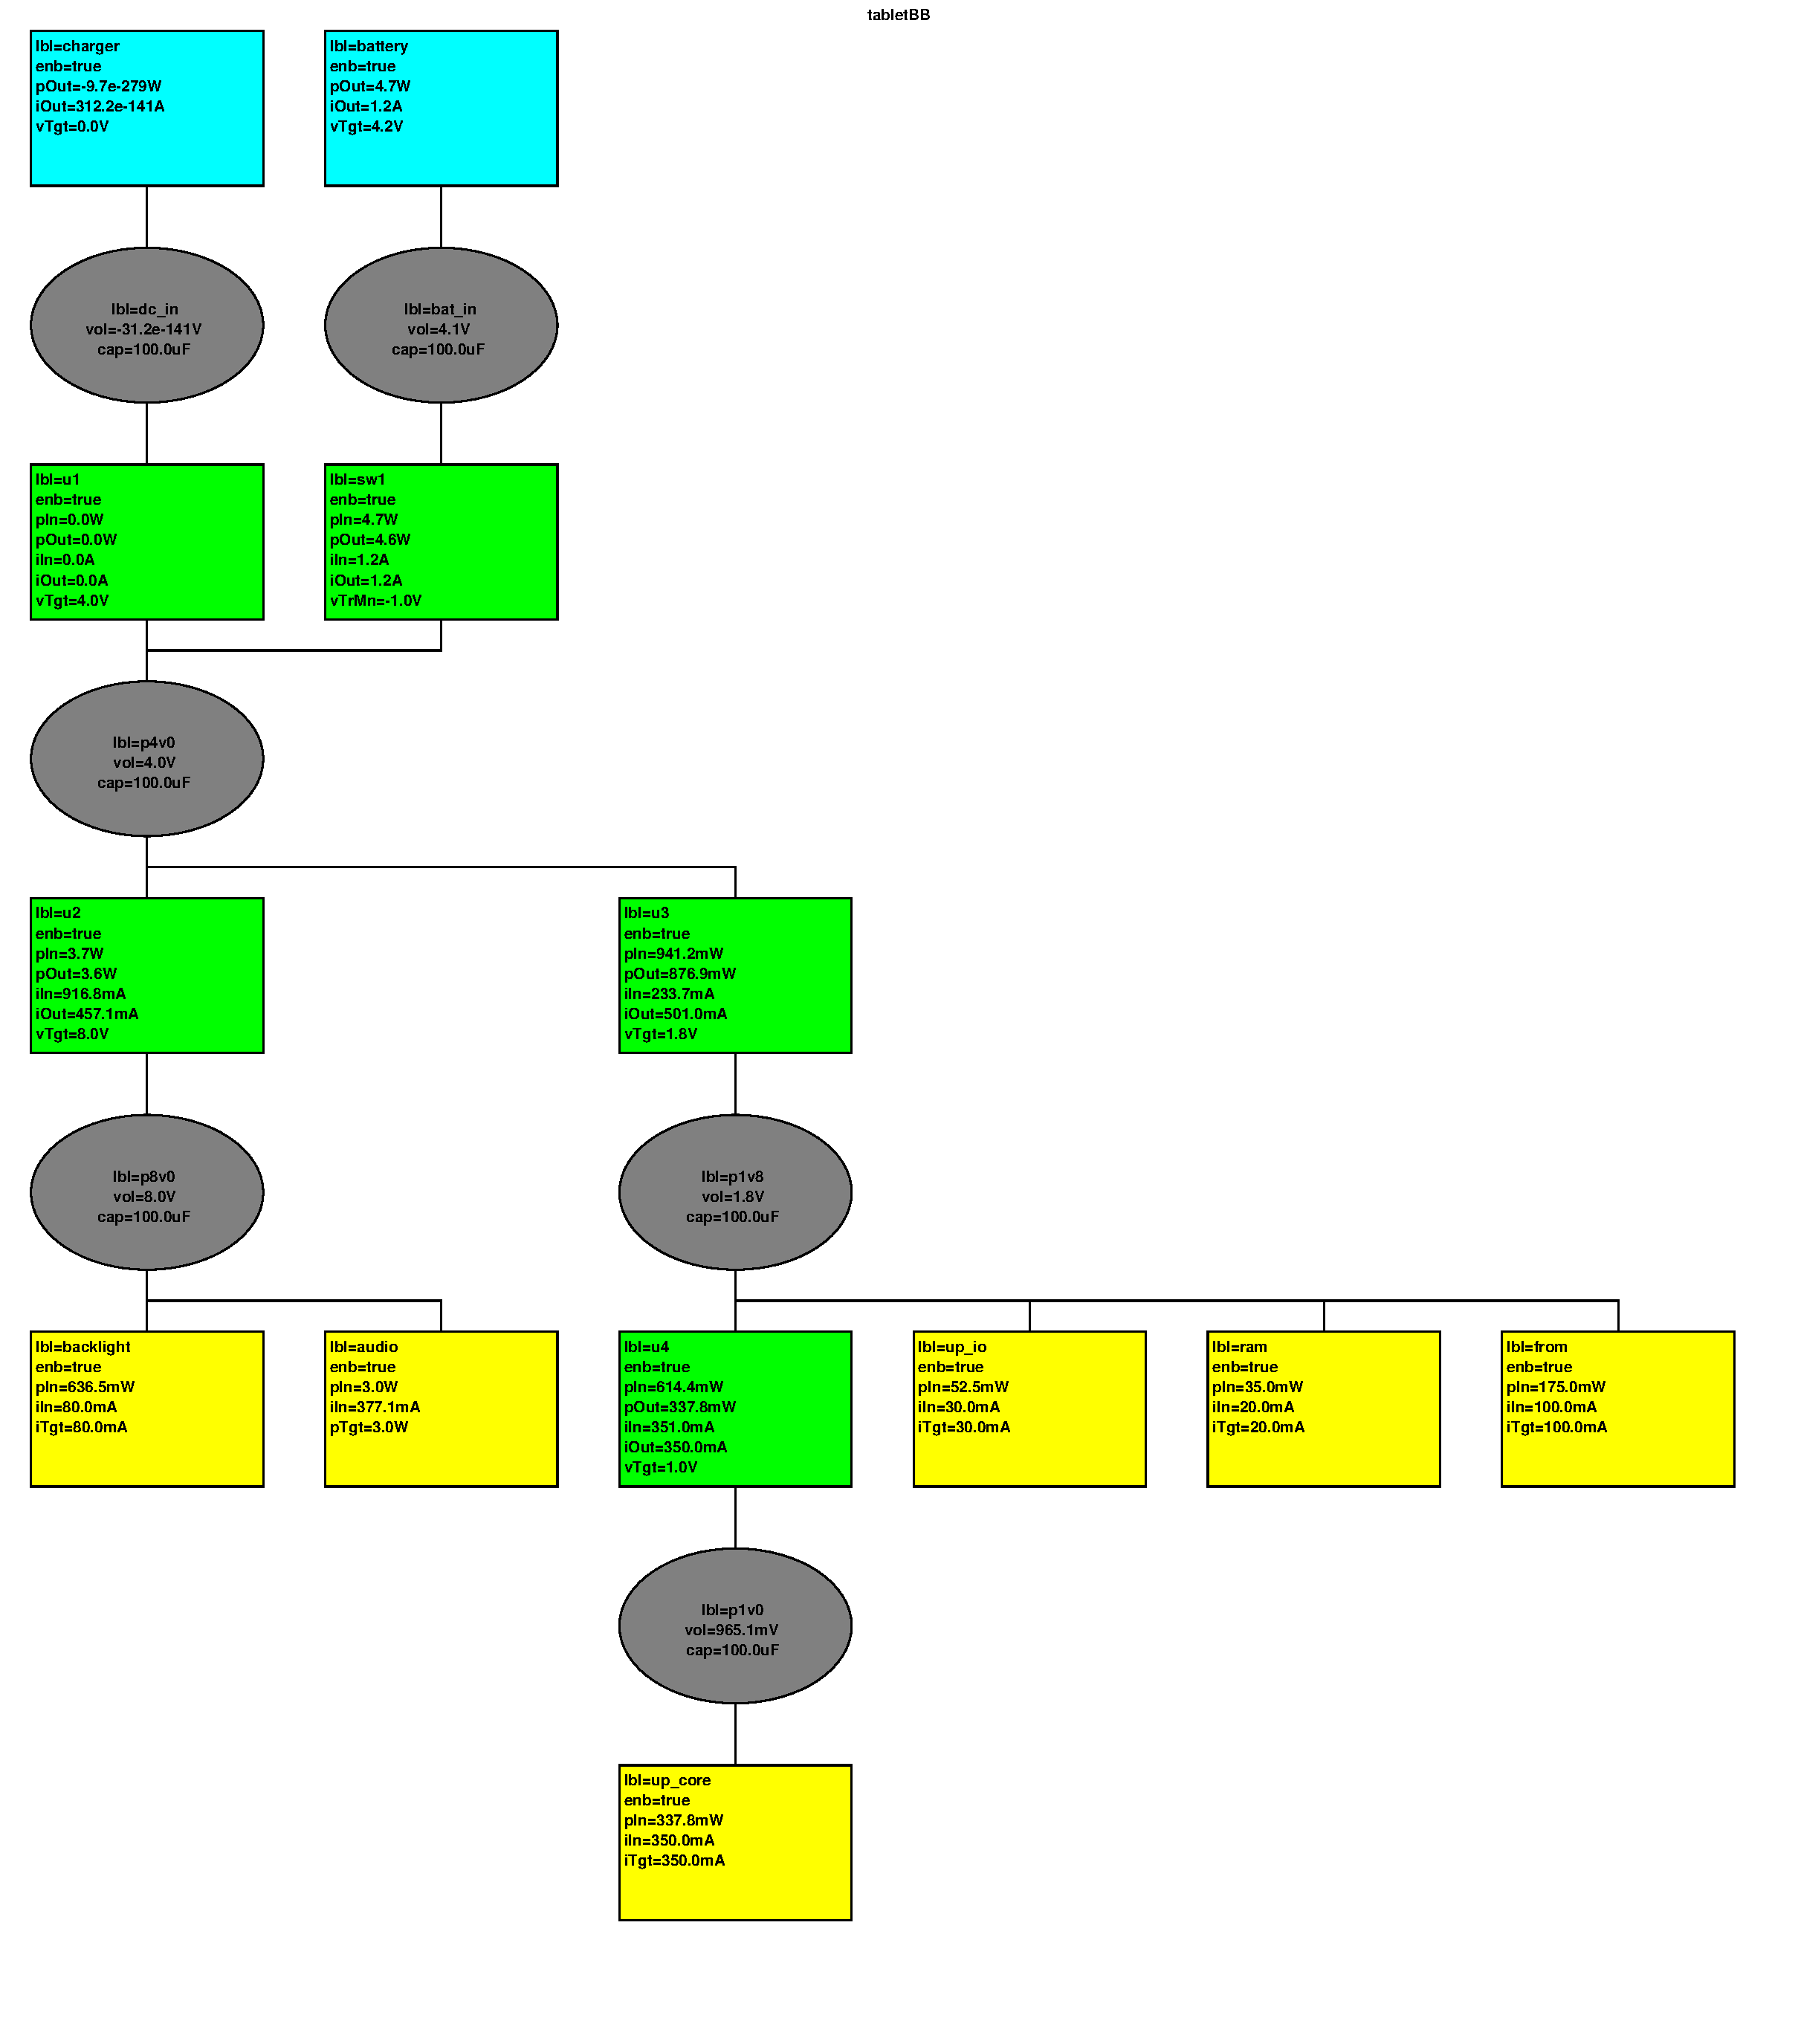
\includegraphics[width=\textwidth]{tabletBB.pdf}\\
Those graphical elements have text showing the value of a subset of the component parameters: label, power, voltage, etc. The label is always printed and also the input and output power for black box. The parameters to show are different depending on the component type. It is possible to customized the parameters to show and the color to use. The diagram is saved on svg or pdf files.\\
Once a transient simulation is run all node voltages and gate currents are saved. A new variable is created (or updated) called TIME. It contains the time points at which the voltage and current values are taken. It is possible to set the number of points to store for the simulation, the default is 1000. Pentode is capable to take a variable for x-axis (usually TIME) and one or more variables for y-axis to plot them on a graph:\\
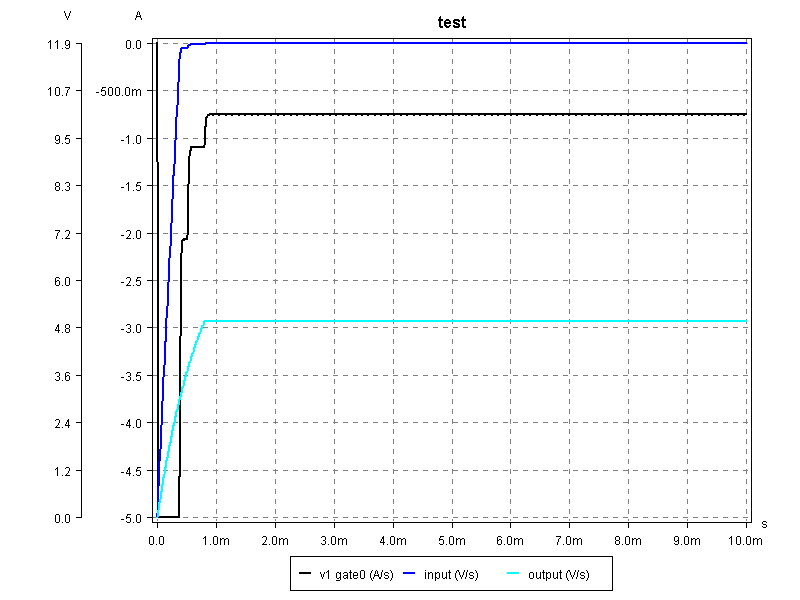
\includegraphics[width=\textwidth]{test.png}\\
The plots are saved on several graphic formats and also in a text file as csv to be manipulated by other programs.\\
It is possible to \emph{print} a component. The print shows its parameter status. It is possible to \emph{list} the components current available on the net list, the variables, etc.  
\subsection{Modify}
The main way to check a power architecture is to try to \emph{modify} some parameter of the components used and simulate again to check the result. It is possible to \emph{delete} components and add new ones just with their definition.\\
One important property is the component \emph{cost}. It is defined by its value and currency. All the components costs can be extracted to compute the BOM (bill of material) amount. In this context all costs are converted to the base currency value.\\
Pentode can define variables. They are single value or arrays with an optional measurement unit. Few variables are automatic made by Pentode, those are in upper case as the variable TIME in a transient simulations: that vector keeps trace of the time at which voltages and currents values are taken. A calculator allows to set a variable value based on the result of computation of other variables. 
There are iteration commands used to \emph{loop} in a condition or iterate \emph{for} a list. Also the basic \emph{if} conditional statements available. \\
The new commands given can be saved updating the net list file or load and execute another file.\\
\section{Syntax}
Pentode read user input in two ways: from a file (ptd extension) and/or interactively by the command line. If the input comes from the command line it is executed just after enter key is pressed. However in few conditions like loops it is not possible to execute the command until all the commands within the loop are written. In that condition it is required to end the lines with + symbol. In that condition Pentode store the lines in its internal buffer until a line without the ending + is found. That is not required for file input.\\
Comment begin with the symbol \# and goes ahead up to the end of line. A comment can fill a whole line or can begin at the end of a command.\\
Every Pentode command has the following structure:\\
name label node1 ... nodeN unlabeled-parameter parameter1 = value1 ... parameterN = valueN\\
Where:
\begin{itemize}
\item name of the command to execute (it may be the definition of component that will be added) 
\item label is the component label or the label required by the command: not all the commands need a label
\item node1 to nodeN if the command is a black box with N gates it is required to define the node1 to nodeN labels the black box gates are linked to. The nodes not already defined are made just before the black box. It is possible to explicitly define the nodes before the black boxes but it is not required. It is done only if the node have not-default parameters.
\item unlabeled-property if available it must be defined just after the node labels
\item property it is possible to set every property to customize the component behavior. The properties can be enter in which ever order. When a property is not set its default value is used. If a property label is not recognized a warning is provided and it is skipped. As a rule Pentode try to go ahead with the input file. There are very few properties without default value which must be explicitly set. Usually the property label are made removing the vocals and using 3 chars: therefore the reverse resistance become rRev. Since there are a lot of properties for every command the help followed by a command name shows the meaning of each property and print followed by a label shows the given component properties settings.
\end{itemize}
\chapter{Components}
This chapter describes the components available on Pentode and their basic properties.\\
\section{Parameter}
A parameter specifies the behavior of a command. It may be the output voltage of a battery or the capacitance of a capacitor.\\ 
Every property has an unique label made by few chars: usually beginning 3 chars of its name skipping vocals. To set a property it is required to write its label, the equal symbol '=', the new value. The property may be of different types: double number, integer number, string, waveform, boolean, list, vector of double, color, money. There are few read-only property which rises an exception if the value is changed. Almost all the properties have a default value that is kept if not set. All properties have a simple help visible looking for the help of the whole command.\\
\subsection{Parameter Types}
There are several parameter types available: double number (double precision real number like 1.1), vector of double, integer, boolean, string, electric component, list, money, option, read only.\\
Double number are used to set parameter for the black boxes internal behavior. It may be the resistance of a resistor or the output voltage of a voltage source. Real number are entered in engineer notation: the value magnitude is followed by one of the following prefix: "f", "p", "n", "u", "m", "", "k", "M", "G", "T" that stands for 10 at power of -15, -12, -9, -6, -6, -3, 3, 3, 6, 9, 12. After the prefix it is also possible to insert the measurement unit (it is used the mksA system, for Ohm it is required to write Ohm because the symbol is not available on the keyboard). The measurement unit is optional however if it is used it must match the correct one otherwise a parse error is generated and the value is discarded. Is is suggested to use the measurement unit when setting parameter to avoid any mistake. As example a 1000 Ohm resistor can be entered as 1kOhm or 1k or 0.001MOhm or 0.001M.\\
A vector of double can be entered with the following syntax: [v1 v2 .... vn |] to understand the meaning see the section about the calculator.\\
An integer value is just an integer value for instance the point of a simulation to save is an integer.\\
A boolean value is true or false, for instance the enable property for the converter is a true of false.\\
A string is a sequence of characters. If the string contains characters it must be contained between double apices ("). String are used as label on the components.\\
An electric component parameter is given by the label of the electric component optionally followed by a dot (.) and one of it parameter. That syntax is used to print and plot components.\\
A list is a list of some other type (of the ones explained before). For instance Plot can print several function on Y axes and they are provided after the plot command separated by commas.\\
A option is a value to be selected between a set of options. For instance the output file for a power tree can be selected between the options pdf and svg. \\
A color parameter represent a color with its red, green and blue components. For instance it is used to set the filling color for power tree drawing.\\
A waveform is used for transient analysis: it describes the output voltage of a source. It can be a simple DC voltage or a PWL (piece wise linear), sinusoidal, trapezoidal or triangular wavers. It can be periodic or not and it can have a set of periods. Please have a look at the manual for further details because it requires to set a lot of parameters.\\
A money used to represent the cost of a component. It is expected a number with dot (.) for separation and ending by a currency. If the currency is not provided the default one is used. To compute the BOM cost all the costs are converted to the default currency. It is possible to set the conversion factor with the \emph{currency} command.\\
A read only parameter is a parameter that cannot be overwritten. It is used to show important internal values depending on other parameter that cannot be overwritten. For instance pOut is the output power computed as output voltage by output current and therefore it cannot be modified. 	\\
\subsection{Calculator}
\subsection{Electrical Components Basic Properties}
There are some properties common to all the electrical components which are explained below:\\
\begin{itemize}
\item name is read-only, it is the name of the component, which is the component command.
\item lbl is read-only, it is the label of the component. It is the unique label of the given component.
\item drwPrm is the list of parameters to plot on the power tree diagram.
\item pltPr is the priority on placement from left to right in the power tree: the lower the sooner is drawn.   
\item drwLnk is a option set to choose how children are linked to father in the power tree diagram
\item cst is the cost of the component, it is used to compute the BOM cost. 
\end{itemize}
The black boxes have some common parameters:
\begin{itemize}
\item enb if the component is enabled: usually there is a little leakage current also when disabled.
\item pLos is read only, it returns the power loss between output and input.
\end{itemize}
\subsubsection{Source Properties}
The source have further common parameters:
\begin{itemize}
\item eff is the efficiency and it is used to compute the power loss.
\item pOut is read only, it computes the output power.
\item iOut is read only, it returns the output current.
\item drwClr is the fill color to be used for the drawing.
\end{itemize}
\subsubsection{Converter Properties}
The source have further common parameters:
\begin{itemize}
\item pIn is read only, it computes the input power.
\item iIn is read only, it returns the input current.
\item pOut is read only, it computes the output power.
\item iOut is read only, it returns the output current.
\item drwClr is the fill color to be used for the drawing.
\item iOff is the input current when the device is disabled. 
\end{itemize}
\subsubsection{Drain Properties}
The source have further common parameters:
\begin{itemize}
\item eff is the efficiency and it is used to compute the power loss.
\item pIn is read only, it computes the input power.
\item iIn is read only, it returns the input current.
\item iOff is the input current when the device is disabled. 
\item drwClr is the fill color to be used for the drawing.
\end{itemize}
\section{Source}
Usually the \emph{sources} are used to provide power to the device however they may drain as well: for instance a current source with a negative current of a voltage source with a voltage lower then the node to which it is linked. Usually sources are not used to drain because their definition is more complex because they can provide arbitrary waveforms.
\section{Converter}
Converter are used to change the power characteristic, usually its voltage, to supply other sections of the device.
\section{Drain}
Drain is the user of the power delivered by source or converter like the display back light or a Bluetooth module.
\chapter{Simulate Commands}
This chapter explains simulation commands.
\chapter{Show commands}
This chapter describe the commands used to show the simulation results.
\chapter{Modify Commands}
This chapter describes the commands to modify the structure.

\chapter{Functions Detailed Description}
\input{help}
\end{document}
